\normaltrue \difficilefalse \tdifficilefalse
\correctionfalse
%\UPSTIidClasse{11} % 11 sup, 12 spé
%\newcommand{\UPSTIidClasse}{11}

\exer{Scooter Piaggio$\star$ \label{B2:16:81}}
%% 
\setcounter{numques}{0}
\UPSTIcompetence[2]{B2-16}
\index{Compétence B2-16}

\index{Scooter Piaggio}
\index{Hyperstatisme}

\ifcorrection
\else
\textbf{Pas de corrigé pour cet exercice.}
\fi


\ifprof
\else
On s'intéresse au système direction du scooter Piaggio.

\begin{figure}[H]
\centering
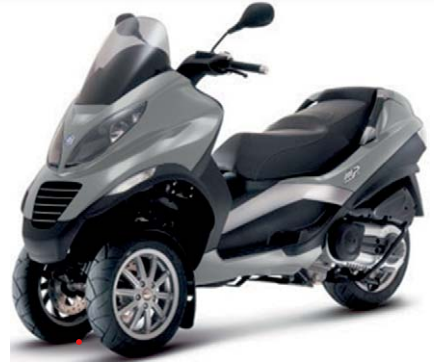
\includegraphics[width=.45\linewidth]{81_01.png}
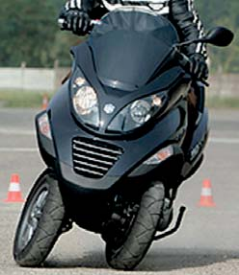
\includegraphics[width=.45\linewidth]{81_02.png}
%\caption{Pince utilisée sur le système ROBOVOLC et schéma cinématique associé \label{fig_23}}
\end{figure} 



\begin{figure}[H]
\centering
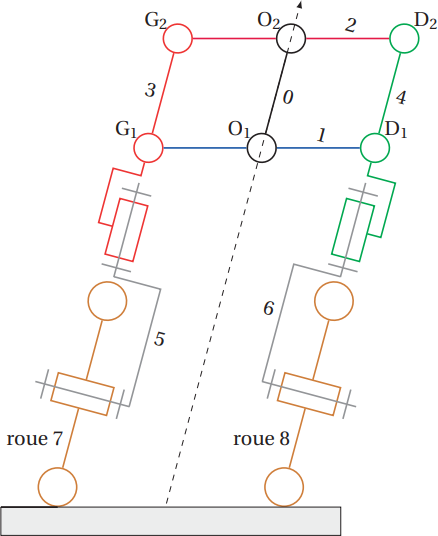
\includegraphics[width=\linewidth]{81_03.png}
%\caption{Pince utilisée sur le système ROBOVOLC et schéma cinématique associé \label{fig_23}}
\end{figure} 
\fi

\question{Réaliser le graphe de liaisons du système de direction. On considèrera le sol comme une classe d'équivalence.}
\ifprof
\begin{center}
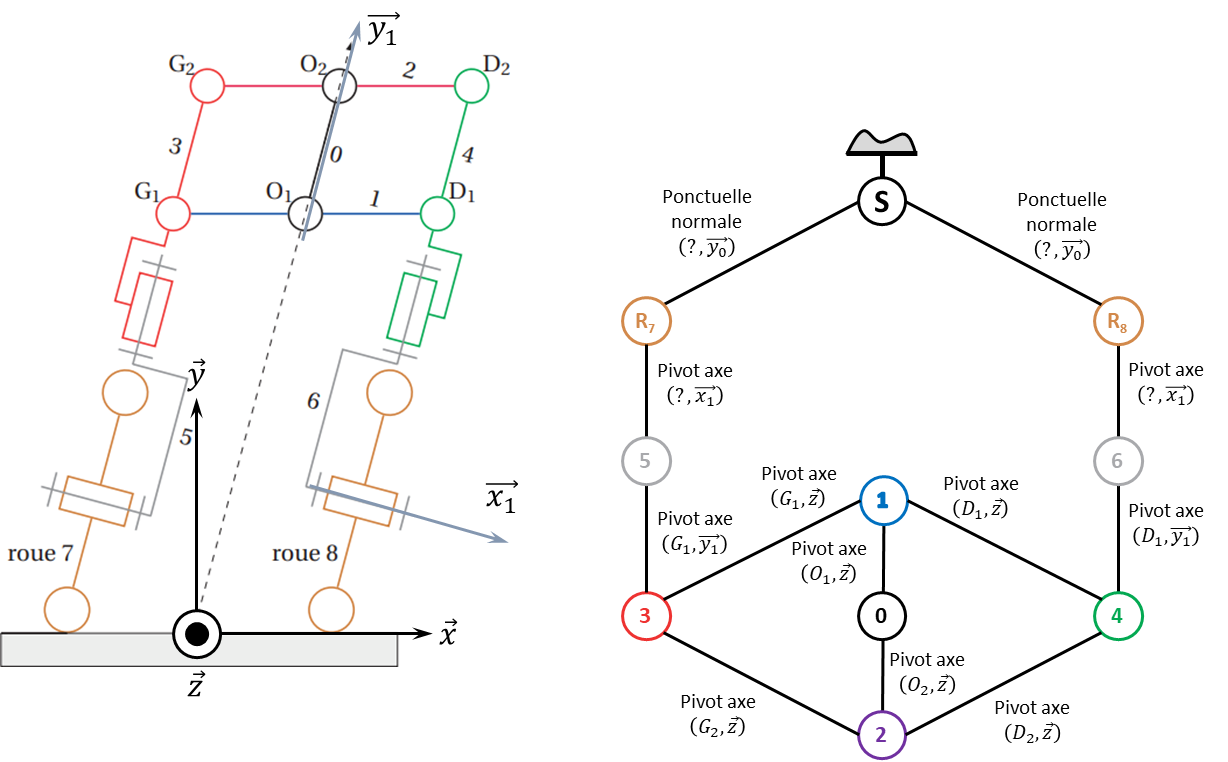
\includegraphics[width=.6\linewidth]{81_01_cor.png}
\end{center}
\else
\fi

\question{Calculer le degré d'hyperstatisme.}
\ifprof
\begin{itemize}
\item $h = m -E_s + I_s$ 
\item $m$ : rotation propre des roues 7 et 8 autour de $\vx{1}$, rotation des roues (7+5) et (6+8) autour de $\vy{1}$,  mouvement du parallèlogramme (1 rotatation), si toutes les liaisons pivots sont bloquées, il reste 2 ponctuelles en parallèle par rapport au sol, soit une liaison linéaire rectiligne (4 mobilités). Au final, $m=9$;
\item $E_S =9\times 6 = 54$;
\item $I_S = 10\times 5 + 2 \times 1 = 52$;
\item $h = 9 -54 + 52 = 7$.
\end{itemize}
\else
\fi
\question{Si le modèle est hyperstatique, modifier le modèle pour le rendre isostatique.}
\ifprof
SI on considère l'ensemble 0,1,2,3,4 : 
\begin{itemize}
\item $h = m -E_s + I_s$ 
\item $m = 1$; 
\item $E_S =4\times 6 = 24$;
\item $I_S = 6\times 5  = 30$;
\item $h = 1 -24 + 30 = 7$. 
\end{itemize}
Tout l'hyperstatisme est donc concentré dans le double parallélogramme. 

On peut remplcer la pivot en $O_1$ par une linéaire annulaire, ce qui supprime 3 inconnues statiques. 
On peut aussi remplaxer les pivots $G_2$ et $D_2$ par des rotules (supprimant ainsi 4 inconnues statiques).
\else
\fi
 

\ifprof
\else

\noindent\footnotesize
 \fbox{\parbox{.9\linewidth}{
 Éléments de corrigé : 
 \begin{enumerate}
\item .
\item $h=7$.
\item .
 \end{enumerate}}}
\normalsize

\begin{flushright}
\footnotesize{Corrigé  voir \ref{B2:16:81}.}
\end{flushright}%
\fi